\section{Introduction}
\subsection*{Objective}
The objective of our project was to take a 3 degree of freedom (DOF) robot manipulator and move an object of unknown mass from an initial state to a specified goal state, and then return the manipulator to its original position.
Three primary methods were experimented with in this project.
The first involved developing a method to estimate the mass matrix of the manipulator, with which a controller was designed to track the arm to the initial state, and back home when the object had been dropped in the goal state.
The second part involved using a Kalman filter to estimate the positions of the initial state, goal state, and the current joint configurations of the manipulator.
The last part was developing an adaptive controller to account for the unknown mass of the object to move it successfully from the initial state to the goal state.

\subsubsection*{Ancillary Tasks}
While not the focus of our project, several other components were required in order to complete the described task.
These include the following:

\begin{itemize}
  \item Path planning algorithm (RRT*)
  \item Trajectory planner
  \item Collision detection
  \item Inverse kinematics to map Cartesian space target into joint space
\end{itemize}

\noindent These items are mentioned here for completeness sake, but are not discussed in details in the report as they were not the primary objective.

\subsection*{Mass Matrix Modeling}
Modeling the mass matrix of a robotic manipulator becomes increasingly difficult as the DOF of the system increase.
Our attempt to avoid this complexity was to model the mass matrix with a neural network.
To further decrease the dimensionality of the problem, it is well understood that the mass matrix is a positive definite (PD) square matrix.
Thus the neural network output only the lower triangle of the matrix, and the remaining values were copied from the output accordingly.
Once the mass matrix neural network was trained, it was used in simulation to develop a trajectory tracking controller.

\subsection*{Uncertainty in Configurations and Perception}
To model the uncertainty in the system, a ``camera'' was assumed to be in the world, providing the position of the initial state and the goal state.
The readings given by the camera sensor were assumed to be noisy, having zero-mean Gaussian white noise about the positions desired.
In order to correctly estimate the desired positions for the arm to reach, a Kalman filter was implemented.
Since this task simply required estimating a stationary target, the filter estimated the position while converging towards the ideal target.

Once the desired positions were established, the arm plotted a trajectory.
However, the joint readings from the arm while moving were also noisy.
These too had a zero-mean Gaussian white noise affecting the readings, with these readings being fed directly to the full-state feedback controller.
A Kalman filter was used once again to reduce the noise from the joint readings.
This task was significantly more challenging though since the joint positions were not stationary, so a dynamic model of the arm was produced to accurately update the Kalman filter throughout the process.

\subsection*{Control Model}
In order to implement the adaptive control in the Julia programming language, we needed a way to account for the adaptation law. This implementation was not initially very straightforward, as the ``simulate!()" function places certain restrictions on the inputs to the control function that we choose. To alleviate this issue, we made the adaptive controller a mutable structure which contains the adaptation parameter as a member. This implementation allows us to continually update the parameter, without having to troubleshoot issues associated with other methods.\\

With this control fully implemented, we then move to the full simulation of the control in which we track the state error and end-effector trajectory.
\begin{figure}[H]
	\centering
	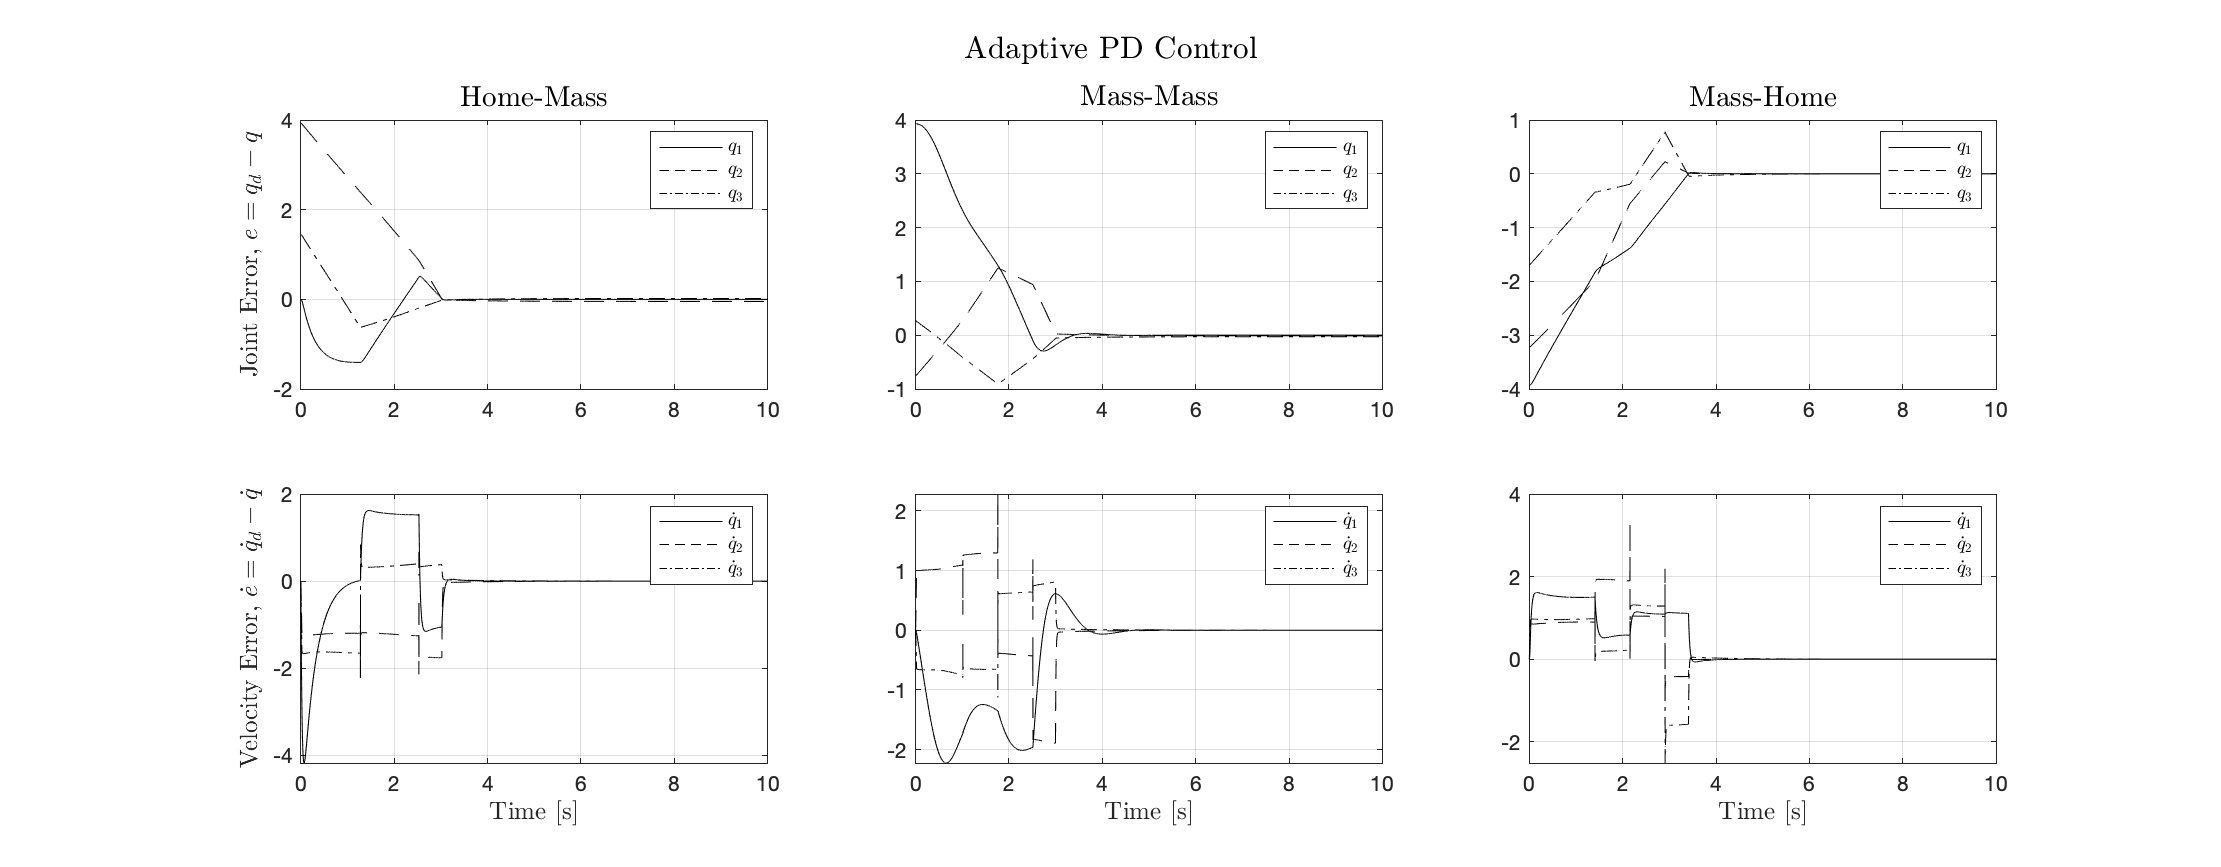
\includegraphics[width=\textwidth]{figures/mass10NNerrAPD.eps}
	\caption{Adaptive controller error in full simulation}
	\label{fig:nnerrapd}
\end{figure}
\begin{figure}[H]
	\centering
	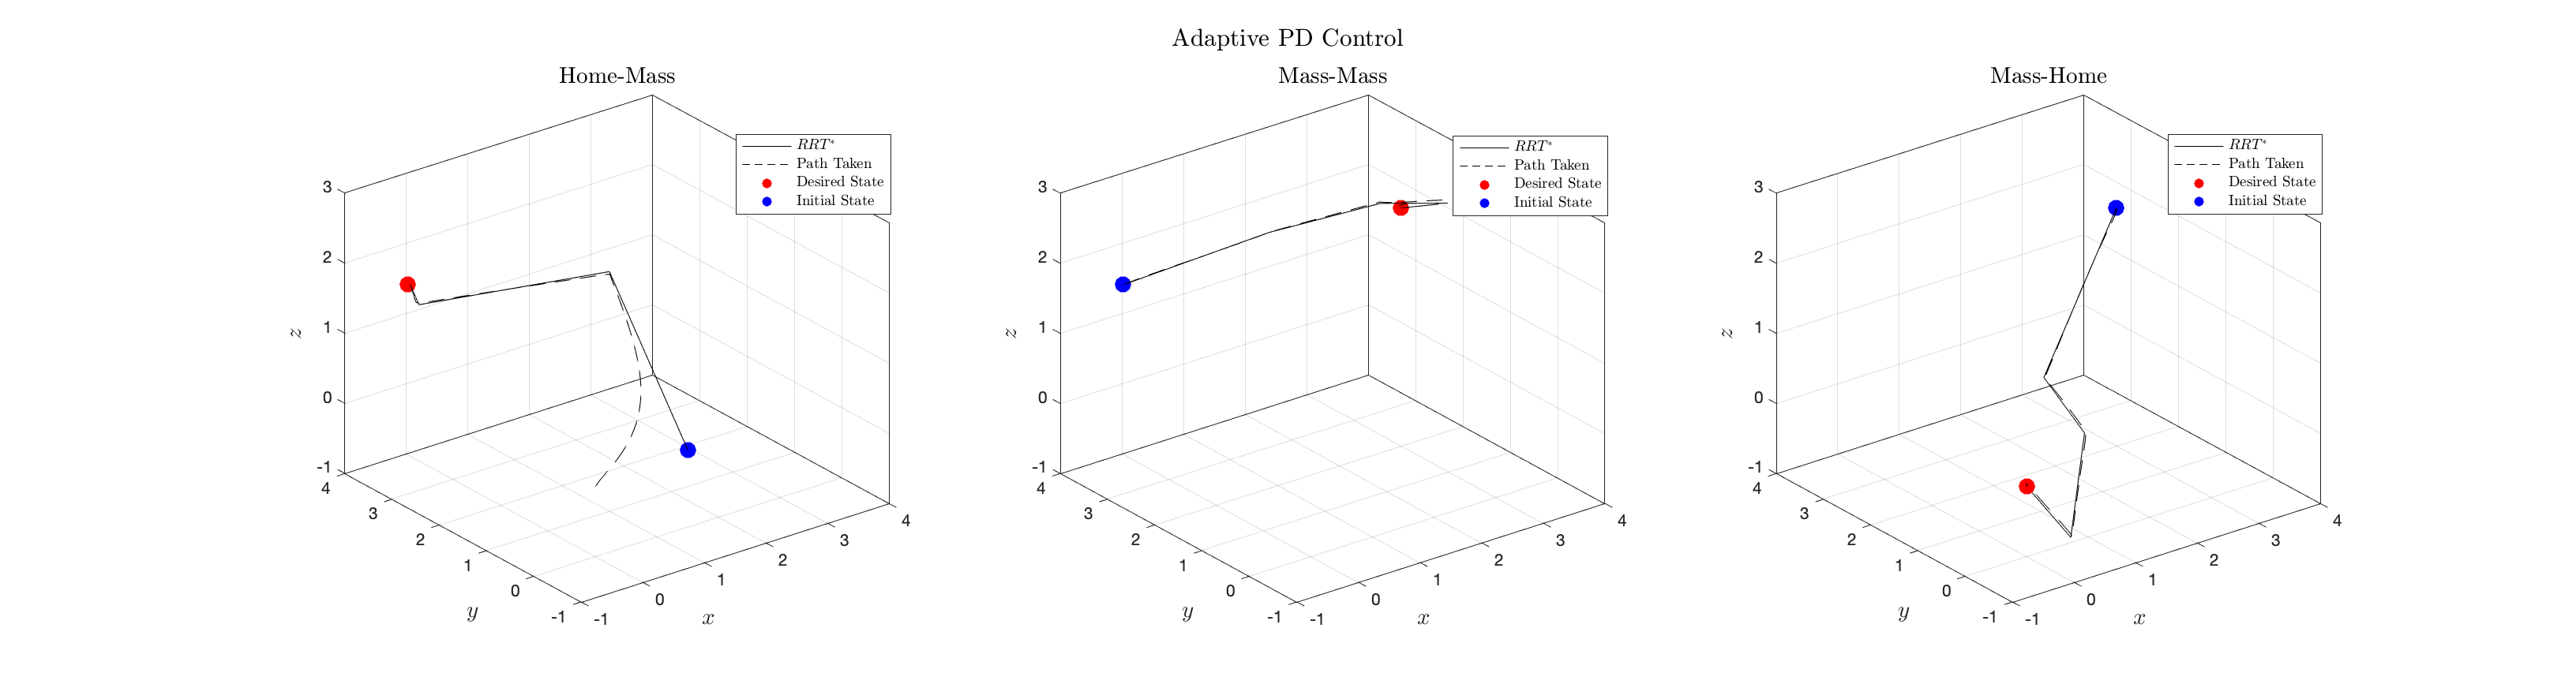
\includegraphics[width=\textwidth]{figures/mass10NNeetrajAPD.eps}
	\caption{End-effector trajectory with adaptive control}
	\label{fig:nntrajapd}
\end{figure}
\noindent We can see from Fig. \ref{fig:nntrajapd} that our initial error results in a false start position, however this error quickly decreases to zero as expected, and the trajectory is followed very tightly for the remainder of the simulation.

We then look at a mass estimated PD model, to observe the effects that an increase in mass has on the control.
\begin{figure}[H]
	\centering
	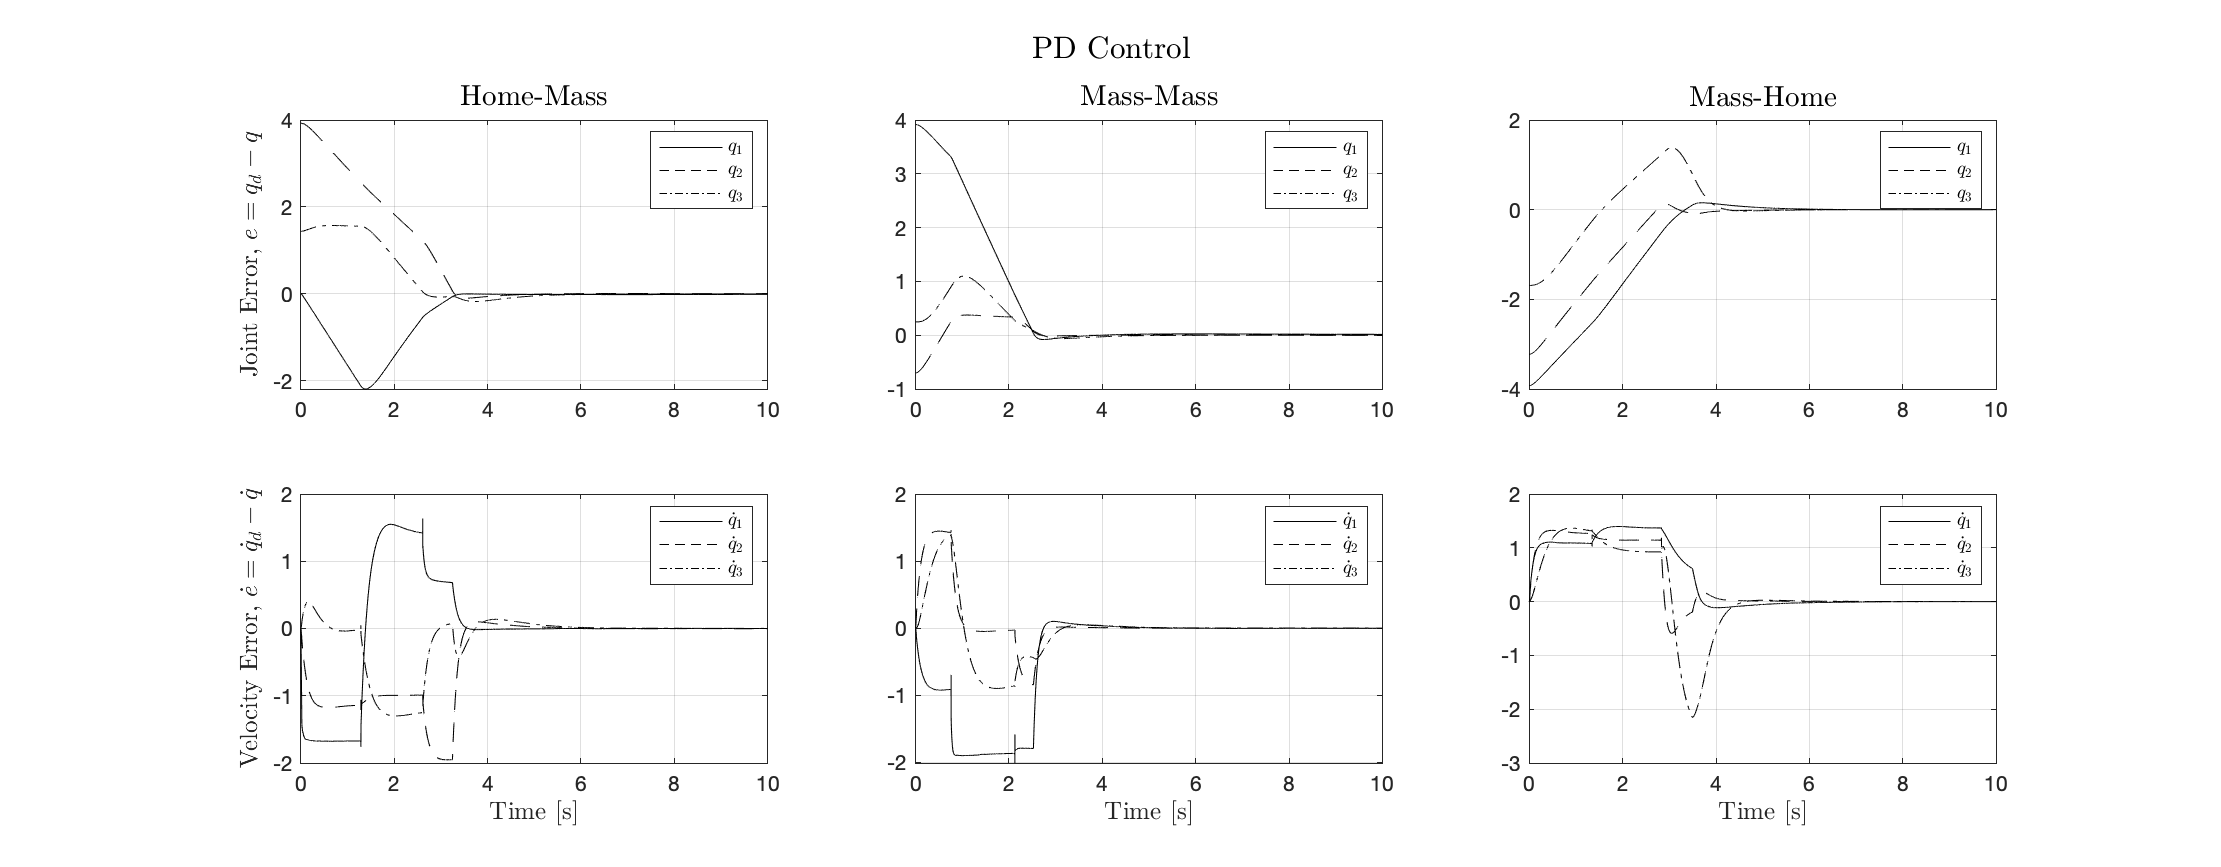
\includegraphics[width=\textwidth]{figures/mass10NNerrPD.eps}
	\caption{Mass estimated PD controller error in full simulation}
	\label{fig:nnerrpd}
\end{figure}
\begin{figure}[H]
	\centering
	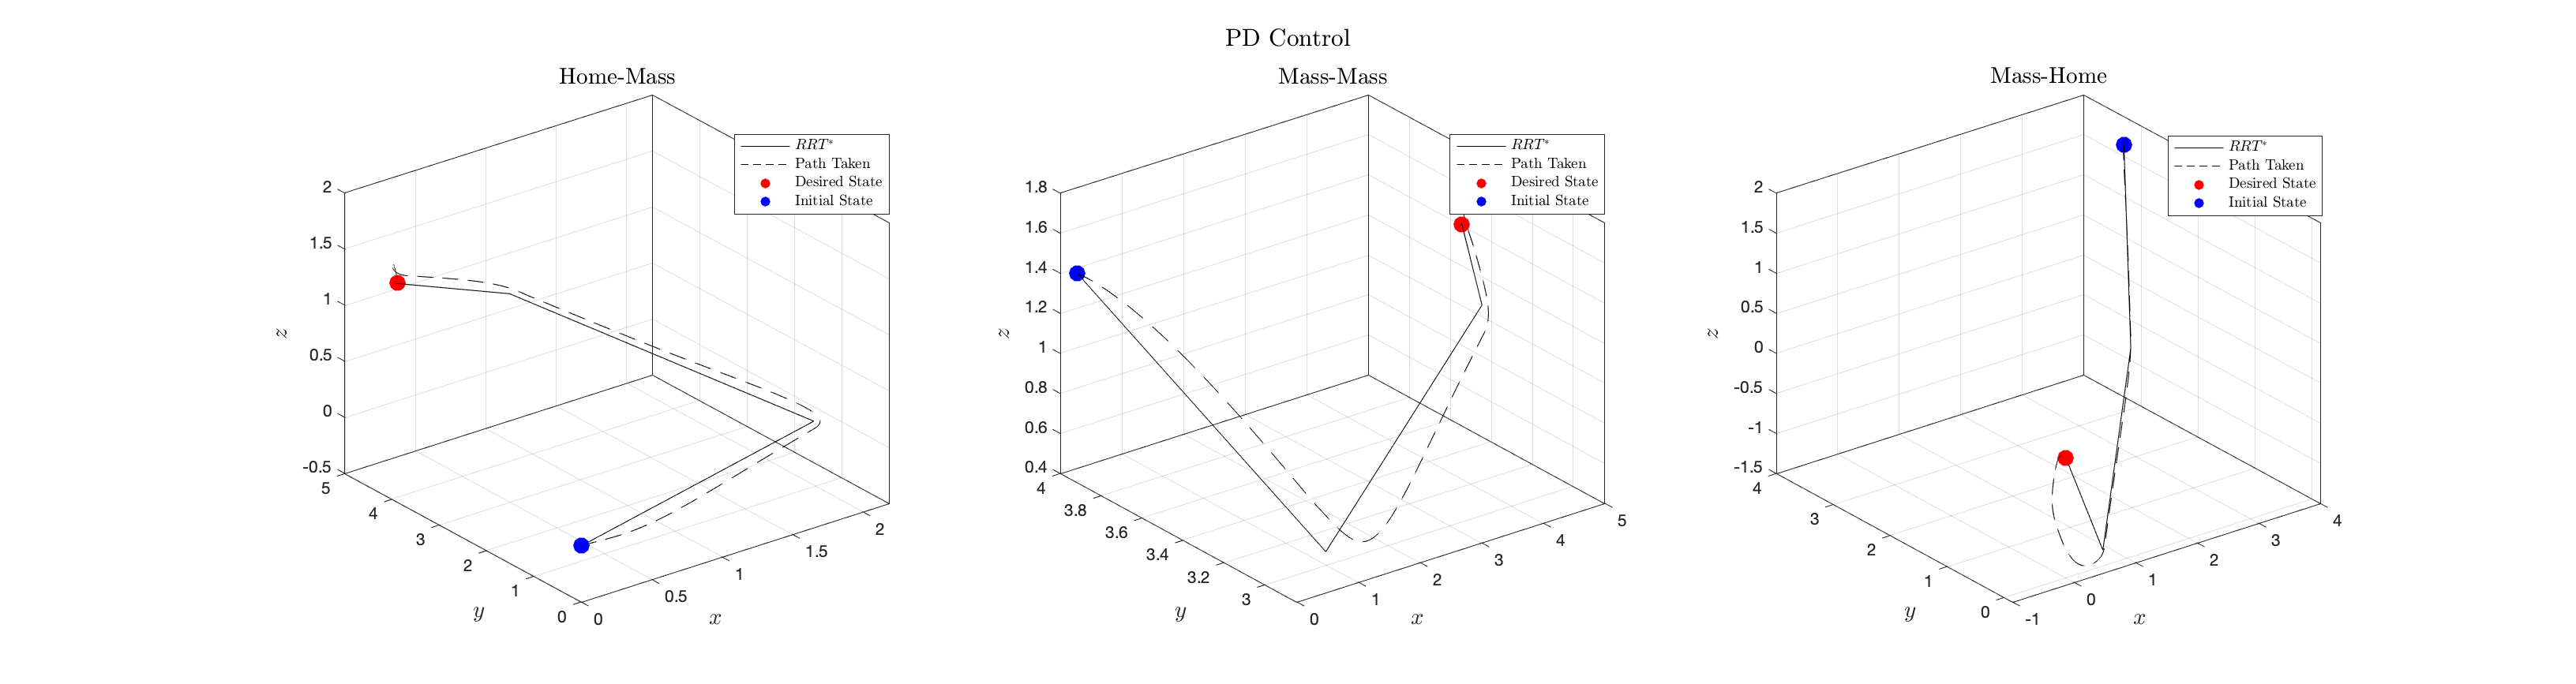
\includegraphics[width=\textwidth]{figures/mass10NNeetrajPD.eps}
	\caption{End-effector trajectory with mass estimated PD control}
	\label{fig:nntrajpd}
\end{figure}
\noindent In contrast to the adaptive model, the mass estimated PD controller places the end-effector in the desired start position.
However, we can easily see from Fig. \ref{fig:nntrajpd} that the PD control is not able to follow the desired trajectory as closely, and once the mass is picked up this issue worsens.

